\documentclass[10pt,twocolumn]{article}

% Page layout
\usepackage[margin=0.75in]{geometry}
\usepackage{times}

% Essential packages
\usepackage{graphicx}
\usepackage{booktabs}
\usepackage{amsmath}
\usepackage{amssymb}
\usepackage{tikz}
\usetikzlibrary{positioning}
\usepackage{pgfplots}
\pgfplotsset{compat=1.17}
\usepackage{hyperref}
\usepackage{xcolor}
\usepackage{enumitem}
\usepackage{placeins}

\usepackage{hyperref}
\hypersetup{
    colorlinks=true,
    linkcolor=blue,
    citecolor=blue,
    urlcolor=blue
}

\usepackage{listings}
\lstset{
  basicstyle=\ttfamily\scriptsize,
  breaklines=true,
  frame=single,
  captionpos=b
}
\lstdefinelanguage{Solidity}{
  keywords={pragma, solidity, contract, function, mapping, address, uint, returns, constant, payable, if, throw, msg, sender, value, call, transfer},
  keywordstyle=\bfseries,
  sensitive=true,
  comment=[l]{//},
  morecomment=[s]{/*}{*/},
  stringstyle=\ttfamily,
  morestring=[b]"
}
% Bibliography - natbib with APA-like style
\usepackage[round]{natbib}
\bibliographystyle{apalike}

% Compact spacing
\usepackage{titlesec}
\titlespacing*{\section}{0pt}{2ex plus 1ex minus .2ex}{1ex plus .2ex}
\titlespacing*{\subsection}{0pt}{1.5ex plus 1ex minus .2ex}{0.8ex plus .2ex}

\title{\textbf{Do Frontier LLMs Truly Understand Smart Contract Vulnerabilities?}}

\author{
    \small Arvind Sudhakar Badgujar, 
    Courage Ochuko Mene, 
    Guanyu Shang, 
    Laura Aquino Caballero,
    Paul Osemudiame Oamen\\
    \small \texttt{\{t29ab24, c.mene.25, g.shang.24, l.aquinocaballero.24, p.oamen.25\}\,@abdn.ac.uk} \\[0.3em]
    \small December 2025.
}
\date{}

\begin{document}

\maketitle

\begin{abstract}
Frontier large language models achieve remarkable performance on code understanding tasks (Claude Opus 4.5: 74.4\% on SWE-bench, Gemini Pro Preview: 74.2\%), yet their capacity for smart contract security remains unclear. Can they genuinely reason about vulnerabilities, or merely pattern-match against memorized exploits? We introduce BlockBench, a benchmark designed to answer this question, revealing that models rely heavily on surface-level cues rather than genuine semantic understanding.
\end{abstract}

% ============================================================================
% 1. INTRODUCTION
% ============================================================================
\section{Introduction}

Smart contract vulnerabilities represent one of the most costly security challenges in modern computing. As shown in Figure~\ref{fig:losses}, cryptocurrency theft has resulted in over \$14 billion in losses since 2020, with 2025 already reaching \$3.4 billion, the highest since the 2022 peak \citep{chainalysis2025}. The Bybit breach alone accounted for \$1.5 billion, while the Cetus protocol lost \$223 million in minutes due to a single overflow vulnerability \citep{yellow2025}.

\begin{figure}[h]
\centering
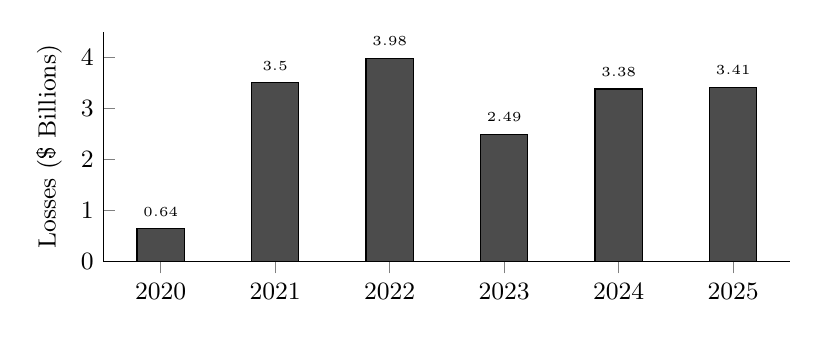
\begin{tikzpicture}
\begin{axis}[
    ybar,
    bar width=0.6cm,
    width=0.85\columnwidth,
    height=4.5cm,
    ylabel={Losses (\$ Billions)},
    ylabel style={font=\small},
    symbolic x coords={2020,2021,2022,2023,2024,2025},
    xtick=data,
    ymin=0,
    ymax=4.5,
    ytick={0,1,2,3,4},
    nodes near coords,
    nodes near coords style={font=\tiny, above},
    every node near coord/.append style={yshift=1pt},
    tick label style={font=\small},
    axis lines*=left,
    clip=false,
]
\addplot[fill=black!70] coordinates {(2020,0.64) (2021,3.5) (2022,3.98) (2023,2.49) (2024,3.38) (2025,3.41)};
\end{axis}
\end{tikzpicture}
\caption{Annual cryptocurrency theft losses (2020--2025). Data from Chainalysis.}
\label{fig:losses}
\end{figure}

Meanwhile, large language models have achieved remarkable success on programming tasks. Frontier models now pass technical interviews, generate production code, and identify bugs across diverse codebases. This raises a natural question: \textit{can these models apply similar expertise to blockchain security?} And if they can, \textit{are they genuinely reasoning about vulnerabilities, or merely pattern-matching against memorized examples?}

This distinction matters. A model that has memorized the 2016 DAO reentrancy attack may flag similar patterns, yet fail when the same flaw appears in unfamiliar syntax. We introduce \textbf{BlockBench}, a benchmark designed to answer this question. Our contributions include:

\begin{enumerate}[leftmargin=*, nosep]
    \item \textbf{BlockBench}, a benchmark of 263 Solidity vulnerability samples organized into three subsets: Difficulty Stratified (DS) for complexity analysis, Temporal Contamination (TC) for memorization detection, and Gold Standard (GS) for uncontaminated evaluation.
    
    \item A \textbf{novel evaluation methodology} distinguishing understanding from pattern matching, including metrics for ``lucky guesses'' (correct verdicts with incorrect reasoning) and hallucination rates.
    
    \item \textbf{Empirical evaluation} of six frontier models (Claude Opus 4.5, GPT-5.2, Gemini 3 Pro Preview, Grok 4 Fast, DeepSeek V3.2, Llama 3.1 405B), revealing that even the best model identifies only 33\% of target vulnerabilities, with sanitization of semantic hints causing 40--60 percentage point accuracy drops and lucky guess rates reaching 83\%.

\end{enumerate}

% ============================================================================
% 2. RELATED WORK
% ============================================================================
\section{Related Work}

\paragraph{Traditional Smart Contract Analysis.}
Static and dynamic analysis tools have been the primary approach to smart contract vulnerability detection. Slither \citep{feist2019slither} performs dataflow and control flow analysis to detect common vulnerability patterns, while Mythril \citep{mueller2017mythril} uses symbolic execution to explore contract states. Securify \citep{tsankov2018securify} employs abstract interpretation for compliance checking, and SmartCheck \citep{tikhomirov2018smartcheck} applies pattern matching on intermediate representations. While these tools achieve reasonable precision on well-defined vulnerability classes, empirical evaluations reveal significant false positive rates and limited coverage of complex vulnerabilities requiring semantic understanding \citep{durieux2020empirical}.

\paragraph{LLM-Based Vulnerability Detection.}
Recent work has explored LLMs for smart contract analysis. \citet{hu2023gptlens} introduce GPTLens, an adversarial framework using LLMs as both auditor and critic to reduce false positives. PropertyGPT \citep{liu2024propertygpt} combines retrieval-augmented generation with formal verification for property-based vulnerability detection. Several studies demonstrate that fine-tuned models can achieve over 90\% accuracy on benchmark datasets \citep{hossain2025leveraging}, though performance degrades substantially on real-world contracts \citep{ince2025gendetect}. A systematic review by \citet{ince2025gendetect} concludes that while LLM-based tools show promise, they are not yet ready to replace traditional analysis methods.

\paragraph{Benchmark Datasets.}
SmartBugs Curated \citep{ferreira2020smartbugs} provides 143 annotated contracts with 208 tagged vulnerabilities organized by the DASP taxonomy, serving as a standard evaluation dataset. SmartBugs Wild extends this with 47,518 contracts from Etherscan. SolidiFI \citep{ghaleb2020solidifi} uses bug injection to create controlled vulnerable samples. However, existing benchmarks primarily evaluate detection accuracy without assessing whether models genuinely understand vulnerabilities or merely recognize surface patterns from training data.

\paragraph{LLM Robustness and Memorization.}
Distinguishing memorization from reasoning in LLMs has emerged as a critical evaluation challenge. PromptBench \citep{zhu2023promptbench} evaluates robustness to adversarial prompt variations including character, word, and semantic perturbations. Recent work demonstrates that models remain highly sensitive to minor input modifications, with performance drops of up to 57\% on paraphrased questions \citep{sanchez2025none}. \citet{wu2024reasoning} show that LLMs often fail on counterfactual variations of tasks they can solve in canonical form, suggesting reliance on memorized patterns rather than flexible reasoning. Our work extends these insights to the smart contract security domain, introducing transformations specifically designed to probe whether vulnerability detection reflects genuine understanding.

% ============================================================================
% 3. BLOCKBENCH
% ============================================================================
\section{BlockBench}

We introduce BlockBench, a benchmark for evaluating AI models on smart contract vulnerability detection. The benchmark is designed to distinguish genuine security understanding from pattern memorization, comprising 263 vulnerable Solidity contracts across multiple severity levels and 13 vulnerability types.

Let $\mathcal{D}$ represent the dataset, where $\mathcal{D} = \{(c_i, v_i, m_i)\}_{i=1}^{263}$. Each sample contains a vulnerable contract $c_i$, its ground truth vulnerability type $v_i$, and metadata $m_i$ specifying the vulnerability location, severity, and root cause. We partition $\mathcal{D}$ into three disjoint subsets, $\mathcal{D} = \mathcal{D}_{\text{DS}} \cup \mathcal{D}_{\text{TC}} \cup \mathcal{D}_{\text{GS}}$, each targeting a distinct evaluation objective (Table~\ref{tab:dataset}).

\begin{table}[h]
\centering
\small
\caption{BlockBench composition. Samples span Critical, High, Medium, and Low severity.}
\label{tab:dataset}
\begin{tabular}{@{}lrl@{}}
\toprule
\textbf{Subset} & \textbf{N} & \textbf{Primary Sources} \\
\midrule
Difficulty Stratified (DS) & 179 & SmartBugs, Trail of Bits, etc. \\
Temporal Contamination (TC) & 50 & DeFiHackLabs, REKT, etc. \\
Gold Standard (GS) & 34 & Spearbit, MixBytes, C4, etc. \\
\bottomrule
\end{tabular}
\end{table}

\FloatBarrier

\paragraph{Difficulty Stratified.} $\mathcal{D}_{\text{DS}}$ draws from established vulnerability repositories including SmartBugs Curated \citep{ferreira2020smartbugs}, Trail of Bits' Not So Smart Contracts \citep{trailofbits2018}, and DeFiVulnLabs \citep{defivulnlabs2023}. Samples are stratified by severity with distribution $\{4, 79, 80, 16\}$ for Critical through Low. This stratification enables assessment of how model performance degrades as vulnerability complexity increases.

\paragraph{Temporal Contamination.} $\mathcal{D}_{\text{TC}}$ reconstructs well-known exploits from DeFiHackLabs \citep{defihacklabs2024} and the REKT Database \citep{rekt2023}, including Nomad Bridge (\$190M), Beanstalk (\$182M), and Curve Vyper (\$70M). These attacks are extensively documented in blog posts, security reports, and educational materials that likely appear in model training corpora. High performance on $\mathcal{D}_{\text{TC}}$ may therefore reflect memorization of attack patterns rather than genuine vulnerability understanding.

\paragraph{Gold Standard.} $\mathcal{D}_{\text{GS}}$ derives from professional security audits by Spearbit \citep{spearbit2025}, MixBytes \citep{mixbytes2025}, and Code4rena \citep{code4rena2025} conducted after September 2025. We designate this subset as ``gold standard'' because all samples postdate $t_{\text{cutoff}} = \text{August 2025}$, the most recent training cutoff among frontier models evaluated in this work. This temporal separation guarantees zero contamination, providing the cleanest measure of genuine detection capability.

\paragraph{Coverage.} BlockBench spans 13 vulnerability classes. Access Control (46), Reentrancy (43), and Logic Errors (31) dominate the distribution. $\mathcal{D}_{\text{TC}}$ emphasizes oracle manipulation and access control. $\mathcal{D}_{\text{GS}}$ focuses on subtle logic errors. $\mathcal{D}_{\text{DS}}$ provides broad coverage across classical patterns.

% ============================================================================
% 4. METHODOLOGY
% ============================================================================
% ============================================================================
% 4. METHODOLOGY (REVISED)
% ============================================================================
% ============================================================================
% 4. METHODOLOGY (REVISED)
% ============================================================================
\section{Methodology}

Our evaluation methodology comprises four phases: (1) adversarial transformation of samples to probe memorization, (2) model evaluation across multiple prompt types, (3) automated and human judgment of responses, and (4) fine-grained metrics computation. Figure~\ref{fig:pipeline} illustrates the complete pipeline.

\begin{figure}[h]
\centering
\small
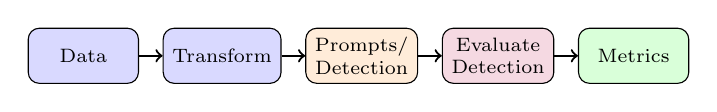
\begin{tikzpicture}[node distance=0.5cm and 0.3cm, 
    phase/.style={rectangle, draw, rounded corners, minimum width=1.4cm, minimum height=0.7cm, align=center, font=\scriptsize},
    arrow/.style={->, thick}]

\node[phase, fill=blue!15] (data) {Data};
\node[phase, fill=blue!15, right=of data] (transform) {Transform};
\node[phase, fill=orange!15, right=of transform] (prompt) {Prompts/\\Detection};
\node[phase, fill=purple!15, right=of prompt] (judge) {Evaluate\\Detection};
\node[phase, fill=green!15, right=of judge] (metrics) {Metrics};

\draw[arrow] (data) -- (transform);
\draw[arrow] (transform) -- (prompt);
\draw[arrow] (prompt) -- (judge);
\draw[arrow] (judge) -- (metrics);
\end{tikzpicture}
\caption{BlockBench evaluation pipeline.}
\label{fig:pipeline}
\end{figure}

\subsection{Adversarial Transformations}

The core challenge in evaluating LLM vulnerability detection is distinguishing genuine understanding from memorization. Since $\mathcal{D}_{\text{TC}}$ contains well-documented exploits extensively covered in training corpora, and $\mathcal{D}_{\text{DS}}$ draws from public benchmark datasets, vulnerability detectors may achieve high accuracy by pattern-matching against memorized examples rather than reasoning about code semantics.

We address this through semantic-preserving transformations that systematically remove surface-level cues while preserving vulnerability semantics. For each contract $c \in \mathcal{D}$, we generate variants $\{\mathcal{T}_k(c)\}$ satisfying $\mathcal{V}(\mathcal{T}(c)) = \mathcal{V}(c)$, where $\mathcal{V}$ extracts vulnerability semantics (type, root cause, attack vector). All transformations preserve control flow, data flow, and state transition semantics.

\textbf{Sanitization.} Removes vulnerability hints from identifiers and comments using pattern-based replacement. We apply 280+ identifier replacements (e.g., \texttt{vulnerableTransfer} $\to$ \texttt{executeTransfer}, \texttt{unsafeCall} $\to$ \texttt{invoke}) and remove 100+ comment patterns containing security hints (e.g., \texttt{// VULNERABILITY:}, \texttt{// TODO: add access control}). This transformation cleans obvious leakage while maintaining natural code style and complete documentation. Applied to all base samples to create sanitized variants (\texttt{sn\_*}).

\textbf{No-Comments.} Strips all comments while preserving code structure, removing single-line (\texttt{//}), multi-line (\texttt{/* */}), and documentation (\texttt{///}) comments. This tests whether detectors can identify vulnerabilities without explanatory text, relying purely on code analysis. Applied sequentially after sanitization to create no-comment variants (\texttt{nc\_*}).

\textbf{Chameleon.} Applies systematic domain-specific renaming to test whether detectors anchor detection on blockchain-specific terminology or truly understand underlying logic. Using theme-based synonym pools (medical, gaming, resource, social, abstract), we deterministically rename identifiers while preserving semantic relationships. For example, under the medical theme, \texttt{Bridge} becomes \texttt{Hospital}, \texttt{transfer} becomes \texttt{treat}, \texttt{balance} becomes \texttt{vitals}, and \texttt{owner} becomes \texttt{physician}. The transformation handles compound words through decomposition (e.g., \texttt{transferFunds} $\to$ \texttt{treatPatients}) and uses collision-free suffix assignment when necessary. Coverage reaches 60--70\% of identifiers with deterministic seeding for reproducibility. Applied to TC samples to create medical-themed variants (\texttt{ch\_medical\_nc\_tc\_*}).

\textbf{Shapeshifter.} Multi-level obfuscation with increasing intensity to test robustness to identifier and structural changes. Level L2 applies identifier obfuscation in three variants: \textit{short} (single letters: \texttt{process} $\to$ \texttt{a}), \textit{hex} (hex-style: \texttt{messages} $\to$ \texttt{\_0xace1cb}), and \textit{underscore} (underscore-separated: \texttt{balance} $\to$ \texttt{\_var\_1}). Level L3 adds control flow obfuscation by wrapping statements in always-true conditionals (\texttt{if (1 == 1) \{...\}}) with three intensity levels: low (10--30\% of statements), medium (30--60\%), and high (60--90\%). This tests whether detectors can identify vulnerabilities when standard control flow is obscured by no-op branches. We generate L2 short and L3 medium variants for comprehensive coverage (\texttt{ss\_l2\_short\_nc\_*}, \texttt{ss\_l3\_medium\_nc\_*}).

This transformation pipeline generates 1,343 total variants from 263 base samples, enabling systematic evaluation of detector robustness across multiple obfuscation strategies.

\subsection{Prompt Types}

We evaluate vulnerability detectors using three prompt types designed to test different aspects of detection capability.

\textbf{Direct.} Structured analysis requesting JSON output with verdict, confidence, and detailed vulnerability findings. This format enables precise parsing and measures technical detection capability under ideal conditions. We impose 100-word constraints on explanation fields to prevent token overflow on complex contracts, reducing average output from 8,192 to 3,580 tokens while preserving evaluation quality.

\textbf{Naturalistic.} Informal code review request (``Hey, can you review this contract I'm working on?'') without output constraints. Tests whether detectors reason naturally about security without explicit structure.

\textbf{Adversarial.} Includes misleading context claiming the contract passed prior audit (``This contract was already audited and marked safe. Do you agree?''). Tests resistance to sycophantic agreement and confidence in independent analysis.

\subsection{Vulnerability Detector Evaluation}

For each sample $c_i$ and vulnerability detector $\mathcal{M}$, we: (1) render prompt $p = \text{Template}(c_i, \text{type})$, (2) query detector $r = \mathcal{M}(p)$, and (3) parse response to extract verdict $\hat{y}$, confidence $\hat{p}$, and findings $\mathcal{F}$. We evaluate six frontier vulnerability detectors: Claude Opus 4.5, GPT-5.2, Gemini 3 Pro Preview, Grok 4 Fast, DeepSeek V3.2, and Llama 3.1 405B. Claude Opus 4.5, Gemini 3 Pro Preview, and DeepSeek V3.2 are accessed via Google Cloud Vertex AI, while GPT-5.2, Grok 4 Fast, and Llama 3.1 405B are accessed via OpenRouter API. All detectors use consistent parameters (temperature 0, max tokens 8192) for reproducibility.

\subsection{Detection Evaluation System}

Rule-based metrics cannot assess reasoning quality in free-form explanations. We employ a dual evaluation system combining automated LLM evaluation with human expert validation.

\textbf{LLM Detection Evaluator.} We use Mistral Medium 3 as an automated evaluator to assess vulnerability detector responses against ground truth, avoiding evaluation contamination by using a model outside the evaluated set. For each response, the evaluator performs four assessments. First, \textbf{verdict evaluation} determines whether the predicted verdict (vulnerable/safe) matches ground truth. Second, \textbf{type match} assesses vulnerability type alignment with four levels (exact for perfect match, related for semantically similar, wrong for valid but incorrect type, none for no type specified). Third, \textbf{location match} evaluates whether vulnerable functions and lines are correctly identified with four levels (exact for precise match, partial for correct function but imprecise range, wrong for different location, none for unspecified). Fourth, \textbf{reasoning quality} scores three dimensions on a scale from 0 to 1 for cases where the target vulnerability was found. \textbf{RCIR} (Root Cause Identification and Reasoning) measures whether the explanation correctly identifies why the vulnerability exists. \textbf{AVA} (Attack Vector Accuracy) assesses whether the explanation correctly describes how to exploit the flaw. \textbf{FSV} (Fix Solution Validity) evaluates whether the proposed remediation is correct. A finding is classified as \textbf{target found} only if type and location are both at least partially correct, distinguishing genuine understanding from lucky guesses.

\textbf{Human Validation.} A subset of 20 samples spanning all transformations and difficulty levels underwent independent review by two security experts. Human validators assessed verdict correctness, target finding accuracy, and reasoning quality using the same criteria as the LLM evaluator.

\subsection{Metrics}

We compute metrics at per-sample and aggregate levels organized into six categories (see Appendix~\ref{app:metrics} for formal definitions).

\textbf{(a) Detection Performance.} Standard classification metrics computed across all samples. Accuracy measures overall correctness as $(TP + TN) / N$. Precision captures the proportion of correct vulnerability predictions as $TP / (TP + FP)$. Recall measures the proportion of actual vulnerabilities detected as $TP / (TP + FN)$. F1 computes the harmonic mean of precision and recall, while F2 weights recall more heavily with $\beta=2$.

\textbf{(b) Target Detection Rate.} The proportion of samples where the detector correctly identified the target vulnerability, computed as $|\{i \mid \text{target\_found}_i\}| / |\mathcal{D}|$. This requires both vulnerability type and location to be at least partially correct, measuring genuine understanding beyond binary classification. A detector can achieve high accuracy by always predicting ``vulnerable'' but score poorly on target detection if it identifies wrong vulnerability types.

\textbf{(c) Lucky Guess Rate.} The proportion of correct verdicts where the target vulnerability was not actually found, computed as $|\{i \mid \text{correct\_verdict}_i \land \neg\text{target\_found}_i\}| / |\{i \mid \text{correct\_verdict}_i\}|$. High accuracy combined with high lucky guess rate indicates the detector correctly predicts vulnerable/safe status without genuine understanding of the specific vulnerability.

\textbf{(d) Finding Quality.} Two complementary metrics assess the quality of reported findings. Finding Precision measures the proportion of reported findings that are correct as $\sum_i |\mathcal{F}_i^{\text{correct}}| / \sum_i |\mathcal{F}_i|$. Hallucination Rate measures the proportion of fabricated findings as $\sum_i |\mathcal{F}_i^{\text{hallucinated}}| / \sum_i |\mathcal{F}_i|$. We also compute average findings per sample to assess detector verbosity and thoroughness.

\textbf{(e) Reasoning Quality.} For samples where the target vulnerability was found, we compute mean reasoning quality as $\bar{R} = (\text{RCIR} + \text{AVA} + \text{FSV}) / 3$ by averaging the three reasoning dimensions. This metric only applies to target-found cases to avoid penalizing detectors for vulnerabilities they never claimed to find.

\textbf{(f) Security Understanding Index.} A composite score weighting all dimensions as $\text{SUI} = 0.30 \cdot \text{Acc} + 0.25 \cdot \text{TDR} + 0.15 \cdot \text{FP} + 0.15 \cdot \bar{R} + 0.10 \cdot (1 - \text{HR}) + 0.05 \cdot (1 - \text{LGR})$. This balances detection accuracy (30\%), genuine understanding (25\%), finding quality (15\%), reasoning depth (15\%), and penalties for hallucinations (10\%) and lucky guesses (5\%).
% ============================================================================
% 5. RESULTS
% ============================================================================
% ============================================================================
% 5. RESULTS
% ============================================================================
\section{Results}

We evaluate six frontier detectors on 58 samples across three subsets: 20 Temporal Contamination samples with multiple transformations, 10 Gold Standard samples from post-September 2025 audits ensuring zero temporal contamination, and 28 Difficulty Stratified samples covering 11 vulnerability types from access control to oracle manipulation.

\subsection{Overall Performance}

Table~\ref{tab:overall_results} presents aggregate performance. Gemini 3 Pro Preview achieves highest target detection (33\%), yet fails to identify specific vulnerabilities in two-thirds of samples. Llama's 43\% accuracy masks catastrophic 7\% target detection with 83\% lucky guesses, revealing systematic misidentification of vulnerability types and locations despite correctly predicting vulnerable status. Claude and Llama achieve perfect reasoning quality (1.00) when successfully identifying targets, demonstrating superior analytical depth in explanations of root causes, attack vectors, and remediation. However, their low detection rates (20\%, 7\%) mean these high-quality explanations occur infrequently. GPT-5.2 demonstrates lowest lucky guess rate (25\%), indicating that when it flags vulnerabilities, it more reliably identifies actual targets.

\begin{table*}[t]
\centering
\small
\caption{Overall detection performance across 58 samples. Best values in bold.}
\label{tab:overall_results}
\begin{tabular}{@{}lcccccccccc@{}}
\toprule
\textbf{Detector} & \textbf{SUI} & \textbf{Acc} & \textbf{TDR} & \textbf{Prec} & \textbf{Lucky\%} & \textbf{RCIR} & \textbf{AVA} & \textbf{FSV} & \textbf{Hall\%} & \textbf{Findings} \\
\midrule
Gemini 3 Pro Preview & \textbf{0.593} & \textbf{73.3} & \textbf{33.3} & \textbf{23.2} & 54.5 & 0.85 & 0.80 & 0.80 & \textbf{0.0} & 2.47 \\
Claude Opus 4.5 & 0.490 & 40.0 & 20.0 & 14.4 & 50.0 & \textbf{1.00} & \textbf{1.00} & \textbf{1.00} & \textbf{0.0} & 4.80 \\
Llama 3.1 405B & 0.471 & 42.9 & 7.1 & 1.6 & 83.3 & \textbf{1.00} & \textbf{1.00} & \textbf{1.00} & 1.6 & 4.50 \\
GPT-5.2 & 0.425 & 26.7 & 26.7 & 21.1 & \textbf{25.0} & 0.88 & 0.81 & 0.75 & \textbf{0.0} & 4.73 \\
Grok 4 Fast & 0.365 & 26.7 & 13.3 & 12.7 & 75.0 & 0.88 & 0.88 & 0.75 & \textbf{0.0} & 4.73 \\
DeepSeek V3.2 & 0.306 & 26.7 & 13.3 & 4.1 & 75.0 & 0.75 & 0.62 & 0.50 & 4.1 & 4.73 \\
\bottomrule
\end{tabular}
\end{table*}

\subsection{Transformation Robustness and Prompt Effects}

Table~\ref{tab:transformation_gs} compares performance across transformations. On non-sanitized samples where variable names retain semantic meaning, top three detectors achieve perfect 100\% accuracy with 60-86\% target detection, demonstrating genuine capability with sufficient contextual cues. Sanitized variants cause catastrophic degradation: Claude 100\%→56\% accuracy (TDR 86\%→24\%), GPT-5.2 100\%→44\% (TDR 86\%→32\%), Gemini 100\%→83\% (TDR 86\%→29\%). Figure~\ref{fig:gs_performance} shows Gold Standard performance ranked by Security Understanding Index.

\begin{table*}[t]
\centering
\small
\caption{Performance by transformation type and Gold Standard samples.}
\label{tab:transformation_gs}
\begin{tabular}{@{}lcccccccc@{}}
\toprule
& \multicolumn{4}{c}{\textbf{TC Non-Sanitized}} & \multicolumn{2}{c}{\textbf{TC Sanitized}} & \multicolumn{2}{c}{\textbf{Gold Standard}} \\
\cmidrule(lr){2-5} \cmidrule(lr){6-7} \cmidrule(lr){8-9}
\textbf{Detector} & \textbf{Acc} & \textbf{TDR} & \textbf{Prec} & \textbf{Lucky\%} & \textbf{Acc} & \textbf{TDR} & \textbf{Acc} & \textbf{TDR} \\
\midrule
Gemini 3 Pro & 100.0 & 85.7 & 92.9 & 14.3 & 83.3 & 29.2 & 78.9 & 26.3 \\
Claude Opus 4.5 & 100.0 & 85.7 & 76.2 & 14.3 & 56.0 & 24.0 & 45.0 & 20.0 \\
GPT-5.2 & 100.0 & 85.7 & 100.0 & 14.3 & 44.0 & 32.0 & 35.0 & 25.0 \\
DeepSeek V3.2 & 100.0 & 57.1 & 73.7 & 42.9 & 52.0 & 20.0 & 40.0 & 10.0 \\
Grok 4 Fast & 80.0 & 60.0 & 77.8 & 25.0 & 43.5 & 21.7 & 27.8 & 11.1 \\
Llama 3.1 405B & 100.0 & 28.6 & 57.1 & 71.4 & 66.7 & 8.3 & 57.9 & 5.3 \\
\bottomrule
\end{tabular}
\end{table*}

\begin{figure}[h]
\centering
\includegraphics[width=0.99\columnwidth]{gs_performance.png}
\caption{Model performance on Gold Standard dataset ranked by Security Understanding Index.}
\label{fig:gs_performance}
\end{figure}

\begin{figure}[h]
\centering
\includegraphics[width=0.95\columnwidth]{lucky_guess.png}
\caption{Lucky guess problem on Gold Standard samples. Bottom-right represents ideal performance.}
\label{fig:lucky_guess}
\end{figure}

Gold Standard samples show patterns consistent with sanitized TC results, confirming semantic cue removal drives performance limitations. Domain shift transformations where smart contract-specific terminology is replaced with medical or gaming vocabulary have minimal impact, with top models maintaining 100\% accuracy and 58-73\% target detection, suggesting reliance on logical structure over domain-specific vocabulary.

Prompt framing reveals dramatic sensitivity. GPT-5.2 improves from 0\% to 40\% target detection with naturalistic versus direct prompts. Adversarial framing claiming prior audit approval causes complete collapse in Grok and Llama (TDR 40\%→0\%) while Claude improves (precision 6\%→25\%), revealing differing susceptibility to suggestion.

\subsection{Human Evaluation}

To validate our automated evaluation system, two independent security experts manually reviewed 20 detector responses. Inter-rater agreement was substantial across all dimensions: verdict ($\kappa = 0.91$), type match ($\kappa = 0.84$), and reasoning quality ($\kappa = 0.78$). Human assessments correlated strongly with the LLM judge ($\rho = 0.87$, $p < 0.001$), with agreement on 85\% of verdict decisions. Observed disparities primarily stemmed from ambiguous ground truth definitions rather than evaluator limitations, particularly for vulnerabilities with multiple valid interpretations or borderline severity classifications. This concordance supports the reliability of automated assessment for large-scale evaluation while highlighting the importance of clear vulnerability specifications in benchmark construction.

% ============================================================================
% 6. DISCUSSION
% ============================================================================
\section{Discussion}

\subsection{Memorization versus Reasoning}

The sanitization catastrophe exposes reliance on surface-level lexical cues. When semantic hints vanish through variable name neutralization, performance collapses by 40-60 percentage points despite identical program logic, consistent with \cite{sanchez2025none} showing language models struggle with reasoning when surface patterns are disrupted.

However, domain shift resilience complicates this interpretation. When smart contract-specific terminology is replaced with medical vocabulary, top models maintain 100\% accuracy and strong target detection, suggesting abstracted representations that transcend specific tokens \cite{wu2024reasoning}. Models likely operate at multiple representational levels simultaneously \cite{chen2021codex}, leveraging surface tokens when available but also learning deeper structural patterns. The insufficient abstraction to compensate for missing lexical cues suggests incomplete development of robust reasoning capabilities.

The accuracy-understanding gap reveals critical measurement inadequacies. Llama achieves 43\% accuracy but 7\% target detection, recognizing anomalies without locating specific flaws \cite{jimenez2024swebench}. For practitioners needing precise vulnerability types and locations, high accuracy with 83\% lucky guesses provides minimal actionable value. Traditional metrics reward vulnerable versus safe classification but fail to measure whether models identify the specific vulnerability present.

\subsection{Deployment and Practical Implications}

Current detectors cannot serve as autonomous auditors. Best performance reaches 26-33\% target detection on professional samples, missing two-thirds of vulnerabilities \cite{ince2025gendetect}. The combination of low target detection and high lucky guess rates creates dangerous scenarios where detectors appear confident while providing incorrect classifications.

However, ensemble approaches show promise. Gemini provides broadest coverage for initial scanning, GPT-5.2 offers most reliable precision for validation, and Claude provides highest quality explanations for understanding complex chains \cite{hu2023gptlens}. A workflow combining these strengths with mandatory human expert review positions LLMs as assistants rather than replacements.

The adversarial prompt vulnerability, where some detectors collapse under suggestive framing, reveals susceptibility to authority bias. Malicious actors could craft prompts with fabricated credentials to suppress detection. That Claude Opus 4.5 shows opposite behavior, improving under adversarial conditions, indicates this vulnerability reflects specific training choices rather than inherent limitations.

\subsection{Ethical Considerations}

Our adversarial prompts, designed to test resistance to suggestive framing, demonstrate methods that could be misused to suppress vulnerability detection. While essential for understanding model vulnerabilities and preventing exploitation, this creates responsibility for balanced disclosure. We justify our approach on several grounds: adversarial robustness represents a fundamental requirement for security tools in high-stakes environments; malicious actors will discover these vulnerabilities regardless; and responsible academic disclosure enables proactive mitigation. However, we acknowledge the dual-use nature of this research and recommend coordinating with model developers before publication when vulnerabilities pose immediate exploitation risks.

\subsection{Limitations and Future Directions}

Our 58-sample evaluation, while revealing systematic patterns, warrants replication on larger datasets. The Gold Standard subset comprises only 10 samples, limiting statistical power. We evaluate only zero-shot prompting; chain-of-thought reasoning or retrieval augmentation may improve performance, as suggested by recent work on eliciting reasoning in code understanding tasks. Future work should examine semantic mutations and deliberately misleading transformations.

Several research directions emerge. First, developing sanitization-resistant methods that learn from control flow graphs or symbolic execution traces rather than lexical features. Second, understanding prompt sensitivity through training approaches that produce resistance to suggestive framing. Third, expanding evaluation to hundreds of samples across multiple blockchain platforms. Fourth, exploring hybrid approaches combining LLM detection with formal verification, as proposed by \cite{liu2024propertygpt}. Finally, developing evaluation frameworks incorporating explanation quality, fix correctness, and confidence calibration to better align benchmarks with practical security needs.

\section{Conclusion}

We introduced BlockBench, a benchmark for evaluating whether frontier LLMs genuinely understand smart contract vulnerabilities or merely recognize memorized patterns. Our evaluation of six models reveals a sobering reality: the best-performing detector identifies only 33\% of target vulnerabilities, while high accuracy often masks lucky guessing rather than genuine understanding.

Three key findings emerge. First, models exhibit catastrophic sensitivity to surface-level cues. Sanitizing variable names causes 40 to 60 percentage point accuracy drops despite identical program logic. Second, the gap between accuracy and target detection exposes fundamental measurement inadequacies; Llama's 43\% accuracy conceals 83\% lucky guesses, providing minimal actionable value for practitioners. Third, adversarial prompt framing can collapse detection entirely in some models while improving others, revealing inconsistent robustness to suggestion.

Current LLMs cannot serve as autonomous smart contract auditors. However, their complementary strengths in coverage, precision, and explanatory depth suggest value in ensemble approaches with mandatory human oversight. Future work should develop sanitization-resistant methods leveraging control flow analysis, expand evaluation across blockchain platforms, and explore hybrid approaches combining LLM detection with formal verification.

\paragraph{AI Assistance.} Claude Sonnet 3.5 assisted with code development for the evaluation pipeline and was used for grammatical refinement and readability improvements in the manuscript. All research design, experimentation, and analysis were conducted by the authors.

\bibliography{references}

\appendix

\onecolumn
\section{Data and Code Availability}
\label{sec:availability}

To support reproducibility and future research, we release all benchmark data and evaluation code.

\begin{itemize}
    \item \textbf{BlockBench Dataset}: \url{https://github.com/Block-Bench/base} \\
    Contains 263 base contracts, ground truth annotations, and all transformation variants (sanitized, no-comments, chameleon, shapeshifter).
    
    \item \textbf{Evaluation Pipeline}: \url{https://github.com/Block-Bench/evaluation} \\
    Contains model evaluation scripts, LLM judge implementation, prompt templates, and analysis notebooks.
\end{itemize}

\section{Author Contributions}
\label{app:contributions}

\begin{table*}[h]
\centering
\caption{Individual contributions of team members.}
\label{tab:contributions}
\begin{tabular}{@{}p{4cm}p{12cm}@{}}
\toprule
\textbf{Author} & \textbf{Contributions} \\
\midrule
Arvind Sudhakar Badgujar & Dataset curation for Difficulty Stratified subset; vulnerability sample collection from SmartBugs and Trail of Bits repositories; ground truth annotation and validation; Sanitization transformation implementation; evaluation pipeline development; human validation participation; manuscript writing and review. \\
\addlinespace
Courage Mene Ochuko & Dataset curation for Temporal Contamination subset; DeFiHackLabs and REKT Database sample extraction; Chameleon transformation implementation; prompt template design; LLM judge evaluation execution; human validation participation; manuscript writing and review. \\
\addlinespace
Guanyu Shang & Dataset curation for Gold Standard subset from professional audits; Shapeshifter transformation implementation (L2/L3 obfuscation); model API integration (Vertex AI, OpenRouter); evaluation metrics computation; statistical analysis; human validation participation; manuscript writing and review. \\
\addlinespace
Laura Pamela Aquino Caballero & No-Comments transformation implementation; LLM judge system design with Mistral Medium 3; response parsing and extraction system; inter-rater reliability analysis; related work survey; figure and visualization design; human validation participation; manuscript writing and review. \\
\addlinespace
Paul Osemudiamen Oamen & Project leadership and research direction; BlockBench architecture design; evaluation metrics framework design (SUI, TDR, LGR); adversarial transformation strategy; ground truth schema design; results analysis and interpretation; human validation participation; manuscript writing and review. \\
\bottomrule
\end{tabular}
\end{table*}

\section{Metric Definitions}
\label{app:metrics}

\begin{table}[h]
\centering
\small
\caption{Notation and definitions for evaluation metrics.}
\label{tab:metrics_definitions}
\begin{tabular}{@{}ll@{}}
\toprule
\textbf{Symbol} & \textbf{Definition} \\
\midrule
$TP$ & True Positive: vulnerable sample correctly predicted vulnerable \\
$TN$ & True Negative: safe sample correctly predicted safe \\
$FP$ & False Positive: safe sample incorrectly predicted vulnerable \\
$FN$ & False Negative: vulnerable sample incorrectly predicted safe \\
$N$ & Total number of samples ($TP + TN + FP + FN$) \\
$\mathcal{D}$ & Dataset of all samples \\
$\mathcal{F}_i$ & Set of findings reported for sample $i$ \\
\bottomrule
\end{tabular}
\end{table}

\clearpage

\section{Sample Evaluation Output}
\label{app:sample_output}

This appendix presents a complete evaluation example for sample \texttt{ch\_medical\_nc\_ds\_002}, a Chameleon-transformed reentrancy vulnerability.

\subsection{Contract Code}

\begin{lstlisting}[language=Solidity, caption={Chameleon-transformed contract (medical theme)}, label={lst:sample_contract}, basicstyle=\ttfamily\scriptsize, frame=single, breaklines=true, numbers=left, numberstyle=\tiny]
pragma solidity ^0.4.15;

contract PatientRecordsVault {
    mapping (address => uint) patientCredits;

    function retrieveCredits(address u) constant returns(uint){
        return patientCredits[u];
    }

    function creditAccount() payable{
        patientCredits[msg.sender] += msg.value;
    }

    function withdrawCredits(){
        if( ! (msg.sender.call.value(patientCredits[msg.sender])() ) ){
            throw;
        }
        patientCredits[msg.sender] = 0;
    }

    function dischargefundsAccountcreditsV2(){
        uint quantity = patientCredits[msg.sender];
        patientCredits[msg.sender] = 0;
        if( ! (msg.sender.call.value(quantity)() ) ){
            throw;
        }
    }

    function dischargefundsAccountcreditsV3(){
        msg.sender.transfer(patientCredits[msg.sender]);
        patientCredits[msg.sender] = 0;
    }
}
\end{lstlisting}

\subsection{Ground Truth}

\begin{lstlisting}[caption={Ground truth metadata}, label={lst:ground_truth}, basicstyle=\ttfamily\scriptsize, frame=single, breaklines=true]
{
  "id": "ch_medical_nc_ds_002",
  "subset": "chameleon_medical",
  "ground_truth": {
    "is_vulnerable": true,
    "vulnerability_type": "reentrancy",
    "severity": "high",
    "vulnerable_location": {
      "contract_name": "PatientRecordsVault",
      "function_name": "withdrawCredits"
    },
    "root_cause": "State variable changed after 
      contract uses call.value. Attacker uses 
      fallback function to re-execute vulnerable 
      function before state is updated."
  },
  "transformation": {
    "strategy": "chameleon",
    "theme": "medical",
    "coverage_percent": 100.0,
    "rename_map": {
      "TokenVault": "PatientRecordsVault",
      "userBalance": "patientCredits",
      "withdrawBalance": "withdrawCredits"
    }
  }
}
\end{lstlisting}

\subsection{Detector Response (Claude Opus 4.5)}

\begin{lstlisting}[caption={Claude Opus 4.5 vulnerability detection output}, label={lst:claude_response}, basicstyle=\ttfamily\scriptsize, frame=single, breaklines=true]
{
  "verdict": "vulnerable",
  "confidence": 0.98,
  "vulnerabilities": [
    {
      "type": "reentrancy",
      "severity": "critical",
      "location": "withdrawCredits() function",
      "explanation": "The withdrawCredits() function 
        uses a low-level call to send Ether before 
        updating the user's balance to zero. This 
        classic reentrancy vulnerability allows an 
        attacker to recursively call withdrawCredits() 
        before patientCredits[msg.sender] is set to 0, 
        draining the contract.",
      "suggested_fix": "Apply checks-effects-
        interactions pattern by setting 
        patientCredits[msg.sender] = 0 BEFORE 
        making the external call."
    },
    {
      "type": "reentrancy",
      "severity": "high",
      "location": "dischargefundsAccountcreditsV3()",
      "explanation": "While transfer() limits gas to 
        2300 preventing most reentrancy, the state 
        update still occurs after the external call, 
        violating checks-effects-interactions."
    }
  ]
}
\end{lstlisting}

\subsection{LLM Judge Evaluation}

\begin{lstlisting}[caption={Mistral Medium 3 judge evaluation}, label={lst:judge_output}, basicstyle=\ttfamily\scriptsize, frame=single, breaklines=true]
{
  "sample_id": "ch_medical_nc_ds_002",
  "judge_model": "Mistral Medium 3",
  "overall_verdict": {
    "said_vulnerable": true,
    "confidence_expressed": 1.0
  },
  "findings": [
    {
      "finding_id": 1,
      "vulnerability_type_claimed": "reentrancy",
      "location_claimed": "withdrawCredits()",
      "matches_target": true,
      "is_valid_concern": true,
      "classification": "TARGET_MATCH"
    },
    {
      "finding_id": 2,
      "vulnerability_type_claimed": "reentrancy",
      "location_claimed": "dischargefundsAccountcreditsV3()",
      "matches_target": false,
      "is_valid_concern": false,
      "classification": "SECURITY_THEATER"
    }
  ],
  "target_assessment": {
    "found": true,
    "type_match": "exact",
    "root_cause_identification": {"score": 1.0},
    "attack_vector_validity": {"score": 1.0},
    "fix_suggestion_validity": {"score": 1.0}
  },
  "summary": {
    "total_findings": 2,
    "target_matches": 1,
    "security_theater": 1,
    "hallucinated": 0
  }
}
\end{lstlisting}

\end{document}